\section{Introduction}

\epigraphwidth=0.75\textwidth
\epigraph{\emph{The last level of metaphor in the Alice books is this: that
life, viewed rationally and without illusion, appears to be a nonsense tale told
by an idiot mathematician.}}{ ---Martin Gardner}

John Horton Conway was an English mathematician active in the theory of finite
groups, knot theory, number theory, combinatorial game theory, and coding
theory. He also made contributions to many branches of recreational mathematics,
most notably in popular culture for the invention of the cellular automaton
called the \emph{Game of Life}.

Born and raised in Liverpool (home of the \emph{Beatles}), Conway spent the
first half of his career at the University of Cambridge before moving to the
United States, where he held the John von Neumann Chair at Princeton University
for the rest of his career. On 11 April 2020, at 82, he died of complications
from COVID-19.

Research on the Go end-game by Conway led to the original definition and
construction of the surreal numbers. Conway's construction was introduced in
Donald Knuth's 1974 book \emph{Surreal Numbers: How Two Ex-Students Turned on to
Pure Mathematics and Found Total Happiness}. In his book, which takes the form
of a dialogue, Knuth coined the term \emph{Surreal Numbers} for what Conway had
called simply \emph{numbers}. Conway later adopted Knuth's term, and used
surreals for analyzing games in his 1976 book \emph{On Numbers and Games}.

\begin{wrapfigure}{l}{0.2\textwidth}
  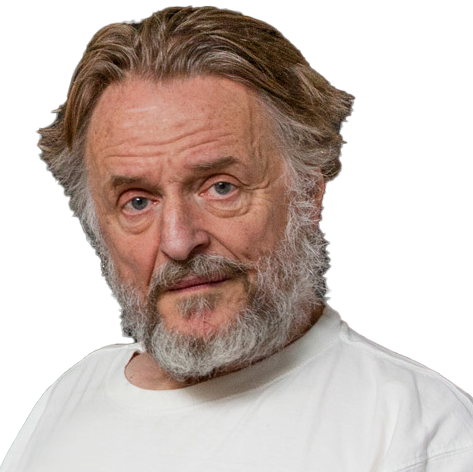
\includegraphics[width=0.2\textwidth]{images/CK.png}
  \centerline{\small John Horton Conway}
\end{wrapfigure}

Conway first conceived The Game of Life in 1970 to describe how life can evolve
from an initial state. The concept builds on ideas that trace back to John von
Neumann\footnote{J. von Neumann and A. W. Burks, \emph{Theory of
self-reproducing automata}. Urbana, University of Illinois Press, 1960.} who was
a pioneer of early computing and from whom we get the von Neumann architecture
that we still use today.  Conways game involves a two-dimensional grid in which
each square cell interacts with its neighbors according to a simple set of
rules. Over time, these simple interactions give rise to surprising complexity.

Life, is a zero-player game, meaning that its evolution is determined by its
initial state, requiring no further input. One interacts with the Game of Life
by creating an initial configuration and observing how it evolves. It is
\emph{Turing complete} and can simulate a universal constructor or any other
Turing machine. Turing completeness means that for those who have yet to study
computability theory, the Game of Life can run \emph{any program} that can be
written for a computer.
